\chapter{Set-Up of Experiment}
%
	The equipment and materials that are needed to perform the experiments are shown in \cref{fig:setup_total}. A detailed
	view of the angular sensor assembly is seen in \cref{fig:setup_detailed}.\par
	Using a desktop computer a serial connection via USB to the \micro C board is established. A serial monitor - \textsc{RealTerm} - is used to
	log the inbound stream send by the \micro C. The relevant settings are listed below:\par
	\begin{itemize}
		\item \SI{9600}{Baud}
		\item On the \texttt{Display} tab, \texttt{Ascii} and \texttt{new Line mode} are checked, \texttt{Direct capture}
		remains un-checked.
		\item COM-Port as assigned by the OS.
	\end{itemize}
	%
	The data is now continuously sent by the \micro C. The data is displayed on the screen. A text file is created in
	which the data is written and saved. Two columns are displayed. The first column contains the time $t$ in seconds, the
	second the number of timer ticks $n$. The current source for the electromagnet is switched on.\par
	Now the setup is completed and the experiments can be started.
	%
	\begin{figure}[h]
		\centering
		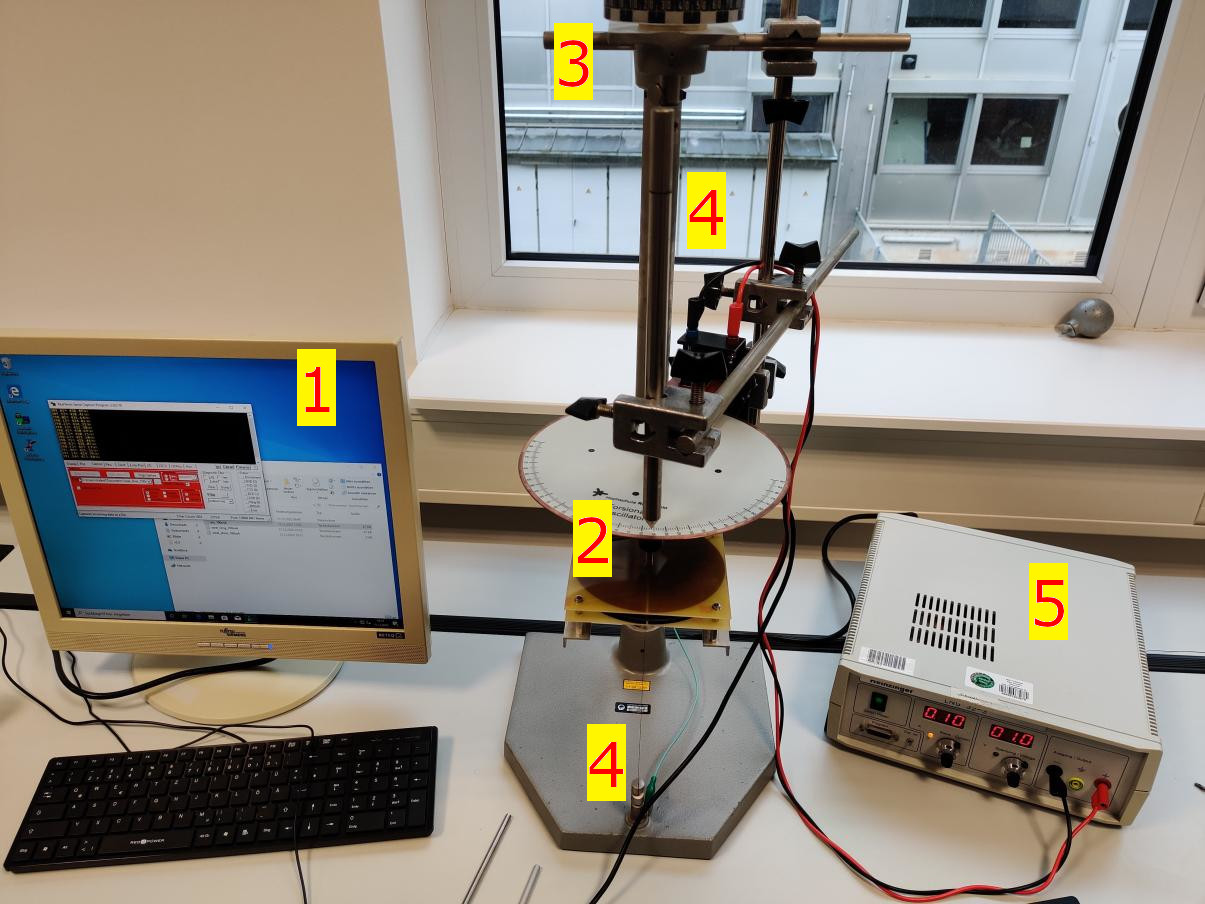
\includegraphics[width=.8\textwidth]{aufbau/setup_total_num.jpg}
		\caption[Equipment used.]{ Equipment and material required for the experiments. 1. Computer running \textsc{RealTerm}, 2. Angular sensor assembly,
		3. Zero adjustment, 4. Torsion wire, 5. PSU in constant current mode powering the eddy current brake.}
		\label{fig:setup_total}
	\end{figure}
	%
	\par
	%
	\begin{figure}[h]
		\centering
		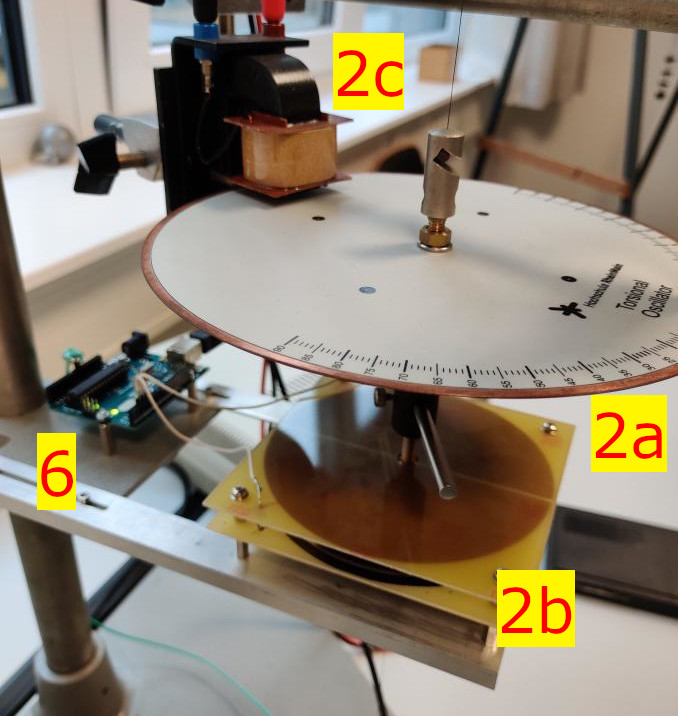
\includegraphics[width=.5\textwidth]{aufbau/setup_pendulum_side_num.jpg}
		\caption[Equipment in detail.]{ Detailed view of the angular sensor assembly. 2a: Copper plate with scale in degree, 2b: Capacitor plates, 2c: Eddy current brake,
		6: \micro C board.}
		\label{fig:setup_detailed}
	\end{figure}
	%